\documentclass[11pt]{article}

\usepackage{bmpsize}
\usepackage[pdftex]{graphicx}
\usepackage{amsmath}
\usepackage{amssymb}
\usepackage{amsthm}
\usepackage{fancyhdr}
\usepackage[margin=2.5cm]{geometry}
\newcommand{\Ohm}{\Omega}
\newcommand{\inv}{^{-1}}
\renewcommand{\part}[1] {\vspace{.10in} {\bf (#1)}}


\pagestyle{fancyplain}


\begin{document}
\title{Lab 4}
\author{David Galbraith}
\maketitle
%COMMENT: In Latex, using the maketitle function will perform all the formatting
%you had set up in the code below in a standard fashion

\normalsize
\begin{abstract} 
In this lab, we used the Leuschner telescope to look at 21cm radiation from the Orion-Eridanus superbubble. Using the data we gathered in 326 pointings, we made plots of the blackbody radiation temperature, hydrogen matter density, and velocity dispersion in the bubble. This gave us some insight into the large-scale structure of this far-off celestial object.

\end{abstract}
%COMMENT: It is customary to use the abstract environment for the
%abstract, and to not include a pagebreak after the abstract prior to
%the introduction in a scientific paper


\lhead{\fancyplain{}{\textbf{Lab 4}}}      % Note the different brackets!
\rhead{\fancyplain{}{David Galbraith}}
\medskip                        % Skip a "medium" amount of space
                                % (latex determines medium is)
                                % Also try: \bigskip, \littleskip

\thispagestyle{plain}

\section{Introduction}
%COMMENT: Sections and subsections have their own format that will make
%the divisions in what you wrote more clear, and will number themselves,
%allowing you to focus more on content rather than order
There are a lot of things in the universe. From our vantage point on Earth, we want to figure out what these things are. Using telescopes, we try to look at them. One of the things we look at is called the 21-cm line. This is the line corresponding to the hyperfine transition of hydrogen, which is when the spins of the proton and electron in a hydrogen atom flip between antiparallel and parallel. When this happens, the hydrogen emits a photon with a frequency of about 1420 MHz, which is a wavelength of about 21 cm. That's why it's called the 21-cm line. This transition is forbidden, so it happens on timescales of ten million years or so for any given hydrogen atom. Therefore, when we observe it, there must be a lot of hydrogen in the region from whence it is coming. This means we can use the 21-cm line to find regions with a lot of hydrogen in them. In addition, the line can be broadened by Doppler broadening. This is when the motion of the atom relative to the observer causes the wavelength to appear different. This gives us information about the velocity dispersion of the hydrogen atoms in the place where we are looking. 

The thing in the universe that we decided to look at this month is the Orion-Eridanus superbubble. A superbubble is a region of space with dimensions in the hundreds of light years that is filled with hot gas. This hot gas came from one or more stars, either from stellar winds or from a supernova. We live in a bubble called the Local Bubble. Over by Orion and Eridanus, there is another bubble: the Orion-Eridanus superbubble. Carl Heiles helped discover it in the 1990s. This bubble takes up the region in the galactic plane from galactic latitude 160-220 degrees and galactic longitude -70 to -10 degrees. This is what we looked at.  

\section{Experiments, Observations, Analysis and Interpretation}
\subsection{Taking and Calibrating Data}
To look at the superbubble, we used a telescope named Leuschner. We told Leuschner to look at the region where the bubble is. To do this, we divided the part of the galactic plane from 160-220 latitude and -70 to -10 longitude into rectangular segments. All of the longitude spacings were 2 degrees, but since the galaxy is curved we only had to space the latitudes 2 / cos($b$) degrees, where $b$ is the longitude. Also, to save time, when we had swept from latitude 160 to 220 for a given longitude, we increased the longitude and swept back from 220 to 160 latitude. This saved much tracking time. But sometimes, the part of the sky where we wanted to look was being blocked, so we could not look at it. This cost us much time and gave us some holes in our images. We picked 2 degrees because that gives two samples per half power beam width. This is important to fulfill the Nyquist Criterion so that we get an accurate image. 
We took four different measurements using the telescope in order to picture the bubble. To isolate the signal of the H1 line, we needed to subtract out the bandpass of our system. To do this, we took one measurement of our signal and one measurement that just consisted of feeding random noise into the system. By subtracting the noise measurement from the signal measurement, what was left over was the signal we are interested in. Except immediately in the vicinity of the H1 line, the spike from that line obscures the underlying shape, so we had to take a shifted measurement as well. The shifted measurement was not centered at the H1 frequency, so we can clearly see the underlying shape there. When we did this shift, it mysteriously changed the gain of the whole system, so we needed to take a measurement of noise in the shifted system as well. We used integration times of ten seconds for the noisee measurements, and we used integration times of a minute for the spectrum measurements. We picked these numbers because the longer integration time (one minute) will give the noise a lot of time to cancel out in the spectrum measurements. In the noise measurements, we want to see noise, so we only used ten seconds so it did not cancel. A graph of all these measurements for a certain point in space appears in Figure \ref{spectra}.

\begin{figure}
\centering
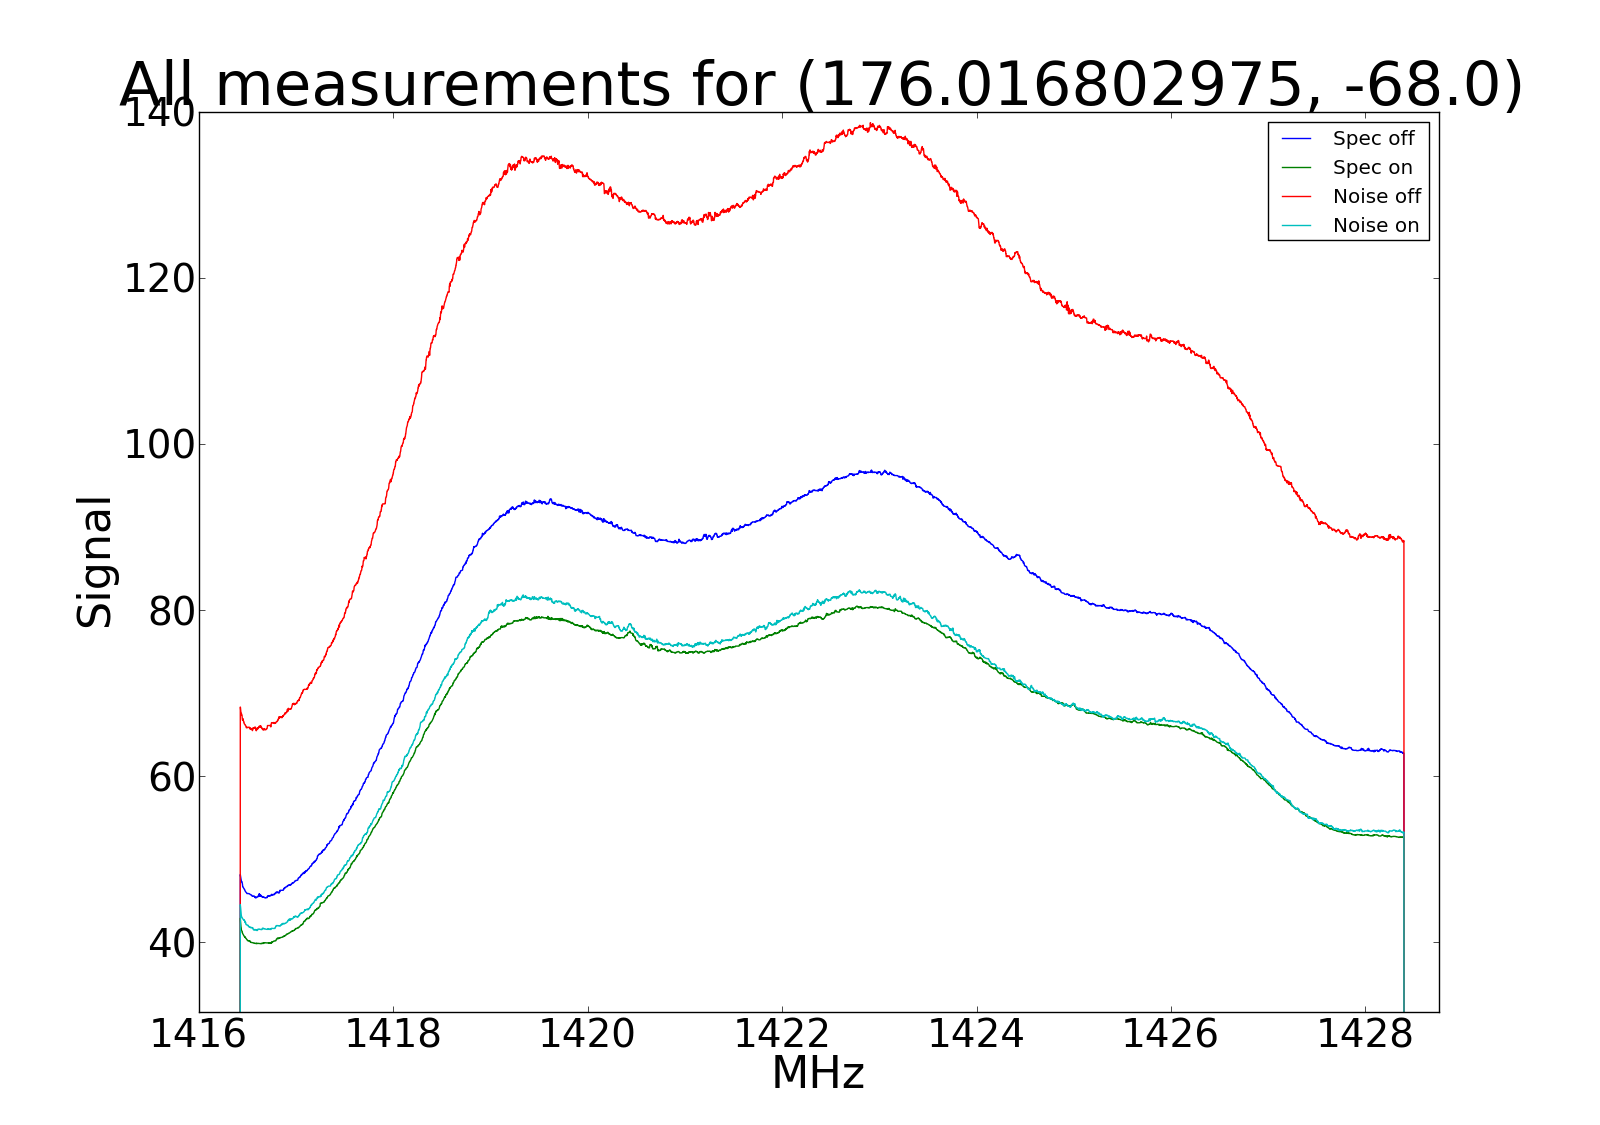
\includegraphics[scale=0.35]{garphs/all}
\caption{This graph displays all four measurements taken with the telescope at a representative galactic coordinate. The blue line shows what we measured when looking at the superbubble. The red line shows the noise corresponding to this measurement. The green line gives the shifted data, and the cyan line is the shifted noise. Note that the power drops to zero outside approximately (1416, 1428) MHz; this is the range in which we told the telescope to measure, because that is where we are likely to see the 21cm line. \label{spectra}}
\end{figure} 

To get usable 21-cm line data, we had to do some data reduction. First, we performed boxcar smoothing on all the data measurements, smoothing out some of the higher-frequency varation. Then, using the ``Cool Method'' of calibration as described in the calibration handout, we calculated the gain as a function of frequency for our telescope circuit, and then we divided that out. The resulting data was still a bit offset from zero and had some filter shape left over, so we took a best-fit polynomial approximation of degree five and subtracted that out of the data. Finally, all that was left was the 21-cm line. The final picture of a representative line appears in Figure \ref{21cm}.

\begin{figure}
\centering
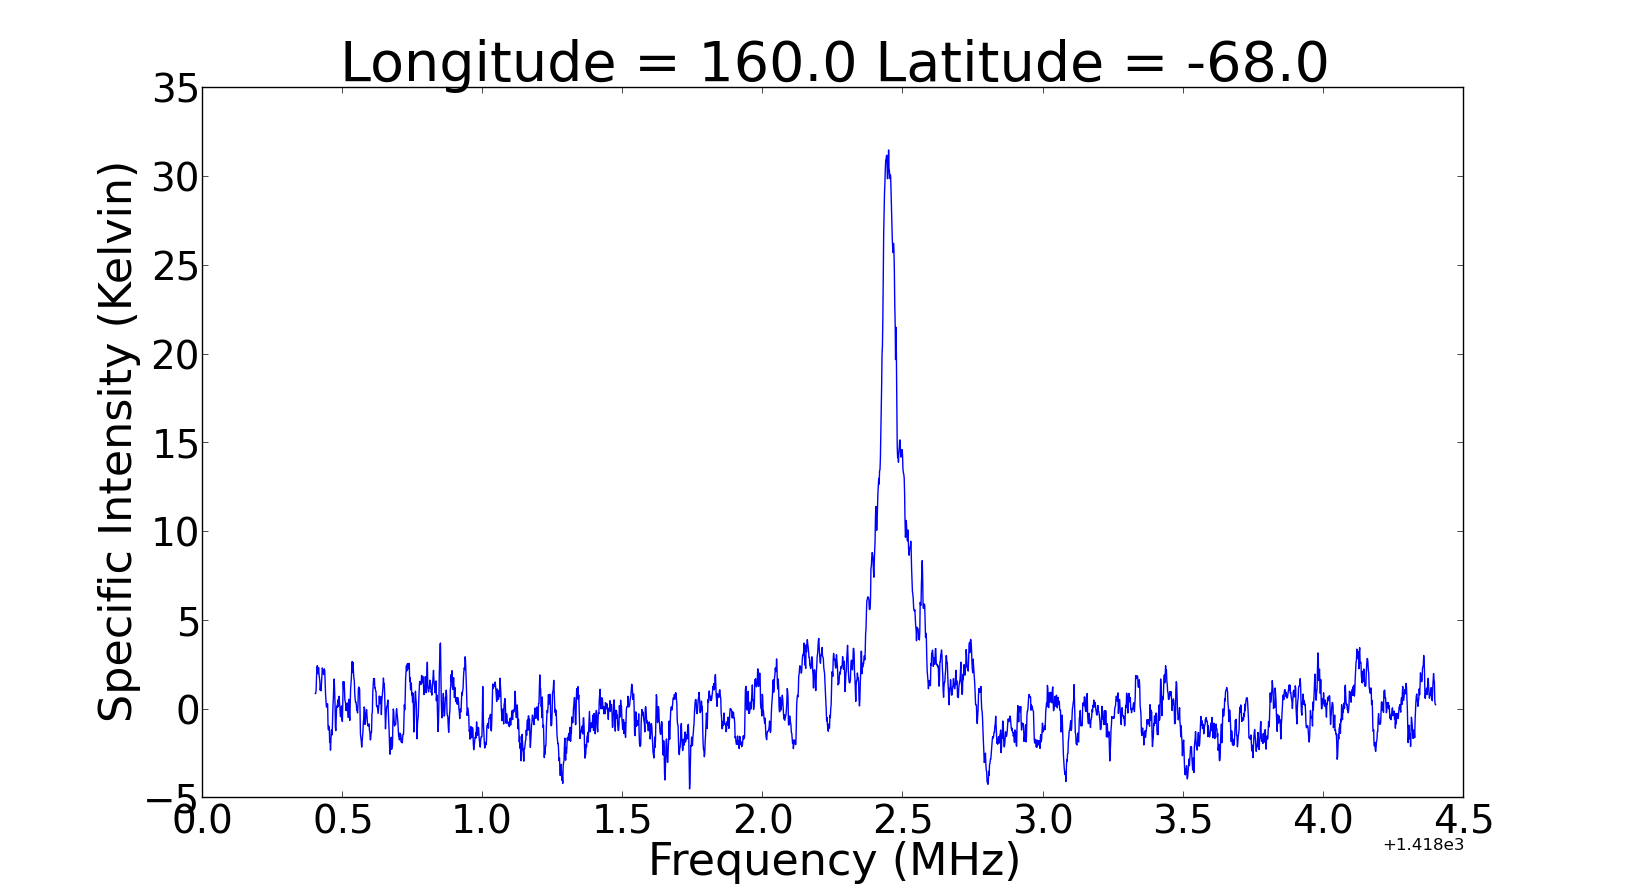
\includegraphics[scale=0.35]{garphs/specint}
\caption{This graph clearly shows the emission line at 21cm (1420 MHz). It stands up way above the noise background, so it's definitely for real. Note the offset of 1418 MHz in the x-axis.\label{21cm}}
\end{figure} 

\subsection{Pictures of the Bubble}
Using these methods, we measured the 21cm emission lines from the bubble at 326 different $(l, b)$ galactic coordinate pairs. These individual points appear in Figure \ref{points}.

\begin{figure}
\centering
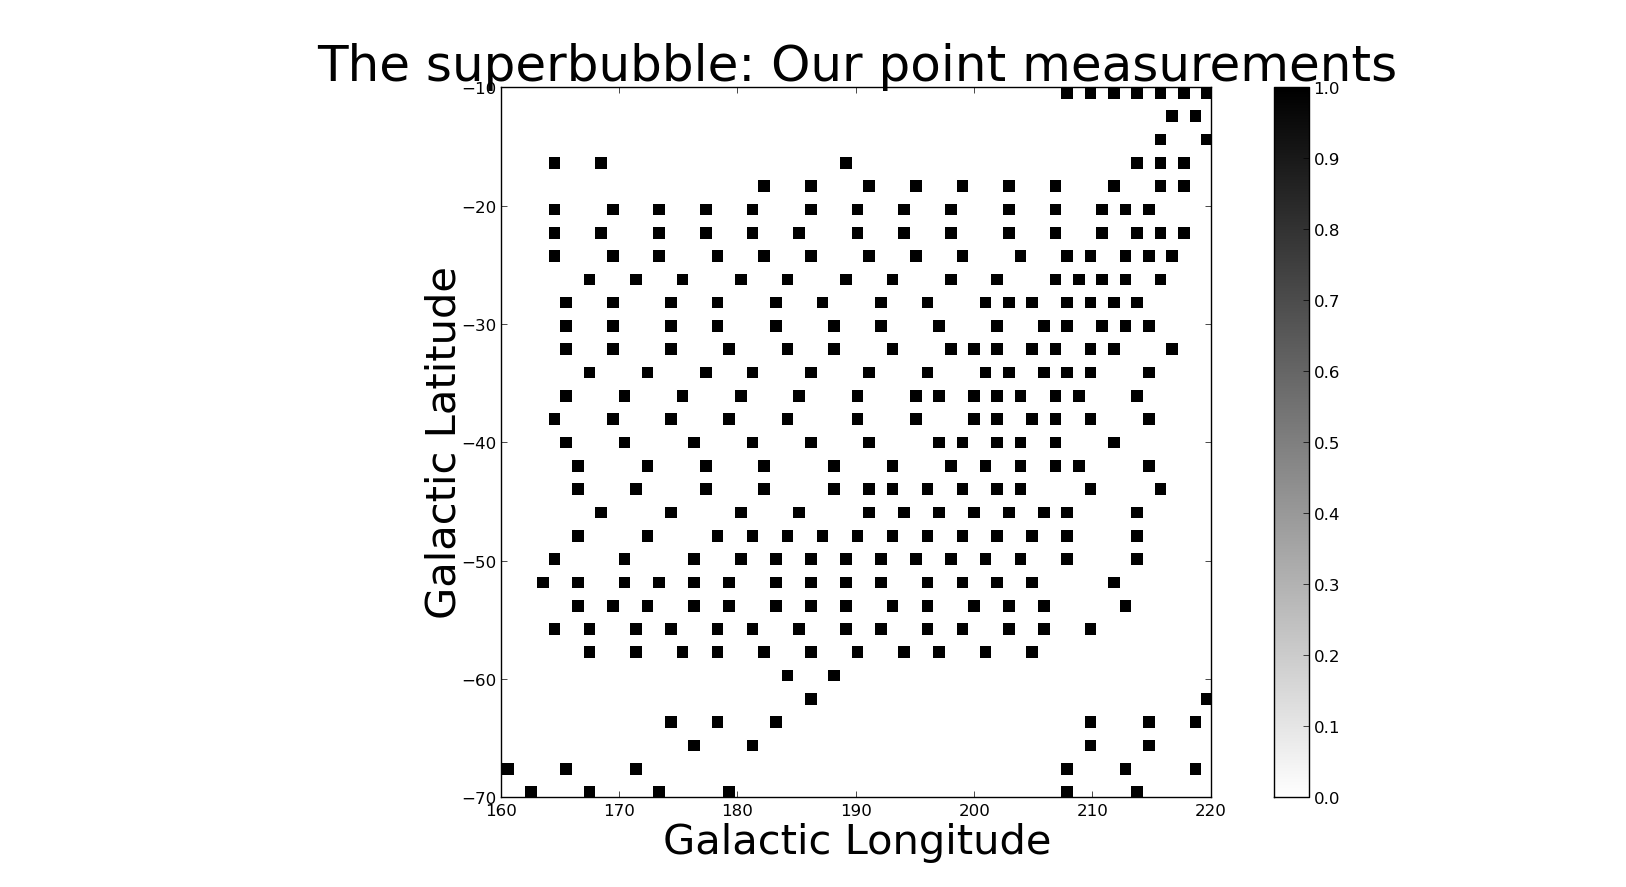
\includegraphics[scale=0.35]{garphs/points}
\caption{This graph shows the 326 points at which we made measurements of the Orion-Eridanus superbubble's 21-cm radio emission. In a perfect world, these would form a grid of squares approximately 4 square degrees in size all throughout the area on the sky where the bubble can be found, which would take around 700 measurements. \label{points}}
\end{figure} 

By plotting the strengths of the transmission lines from these points, we can make a plot of the equivalent black-body temperature for the observed radiation. We fill in the area between the points we observed at using Gaussian FFT convolution. This plot appears in Figure \ref{blackbody}.

\begin{figure}
\centering
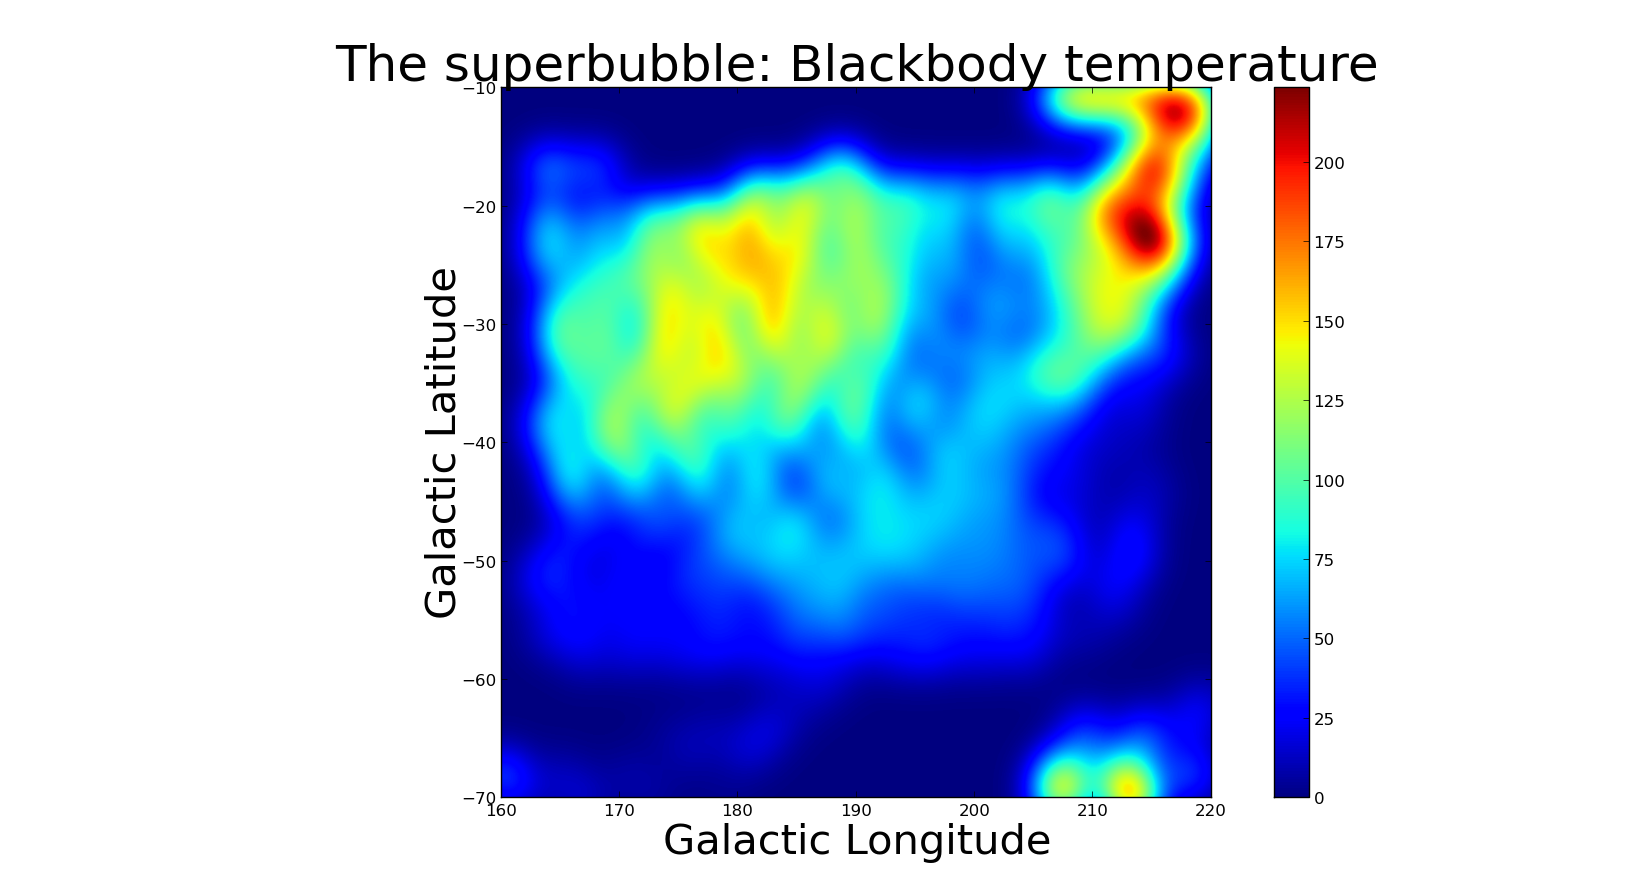
\includegraphics[scale=0.35]{garphs/blackbody}
\caption{This graph maps the blackbody temperature of the Orion-Eridanus superbubble as a function of latitude and longitude. We smoothed using a Gaussian centered in the center of the screen with standard deviation 3.1 degrees. The absolute values of the measurements are not reflective of the temperatures, since our measurements differ from the actual values of the temperatures by a proportionality constant, but the relative shadings do reflect the different temperatures of the parts of the superbubble.\label{blackbody}}
\end{figure} 

Using the equations towards the end of the lab manual, we are able to make a map of the mass of hydrogen seen by the telescope at each point in the bubble, using formula 7 from the lab manual. This graph appears in Figure \ref{hydrogen}.

\begin{figure}
\centering
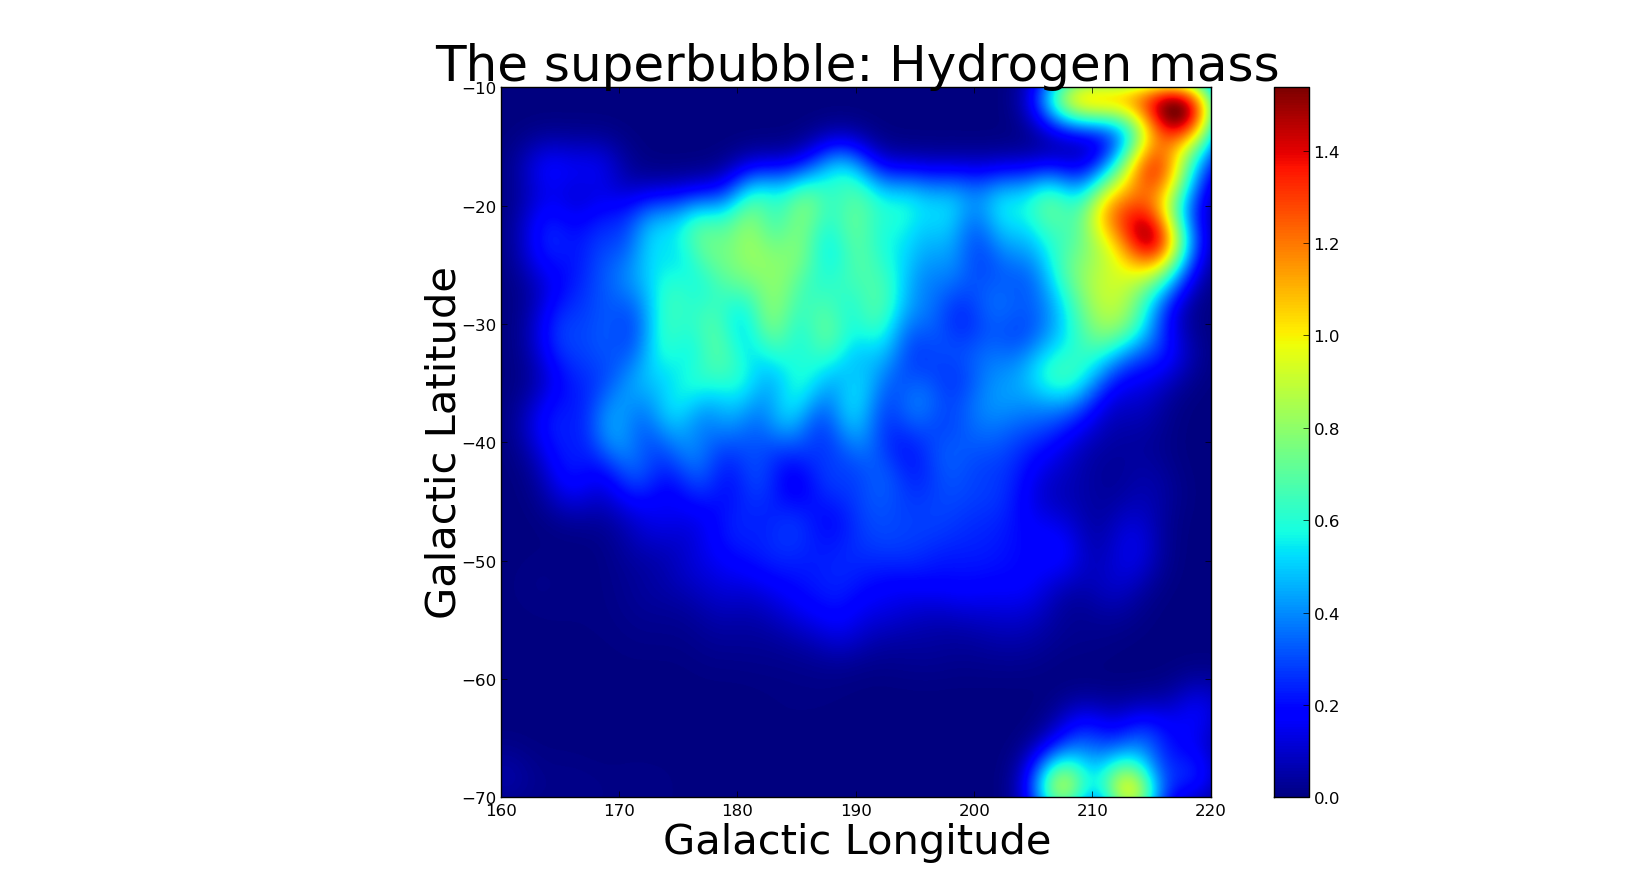
\includegraphics[scale=0.35]{garphs/hydrogen}
\caption{This graph maps the hydrogen density of the Orion-Eridanus superbubble as a function of latitude and longitude. We smoothed using a Gaussian centered in the center of the screen with standard deviation 3.1 degrees. We approximated the distance to the bubble as 400 parsecs and used a beam width $\Omega_b$ of 4 degrees. As above, only the relative measurements have significance. \label{hydrogen}}
\end{figure} 

Finally, we used the formula $v = -\Delta\nu / 4.73$ km/s to make a plot of the velocity of the parts of the superbubble. This appears in Figure \ref{velocity}. 

\begin{figure}
\centering
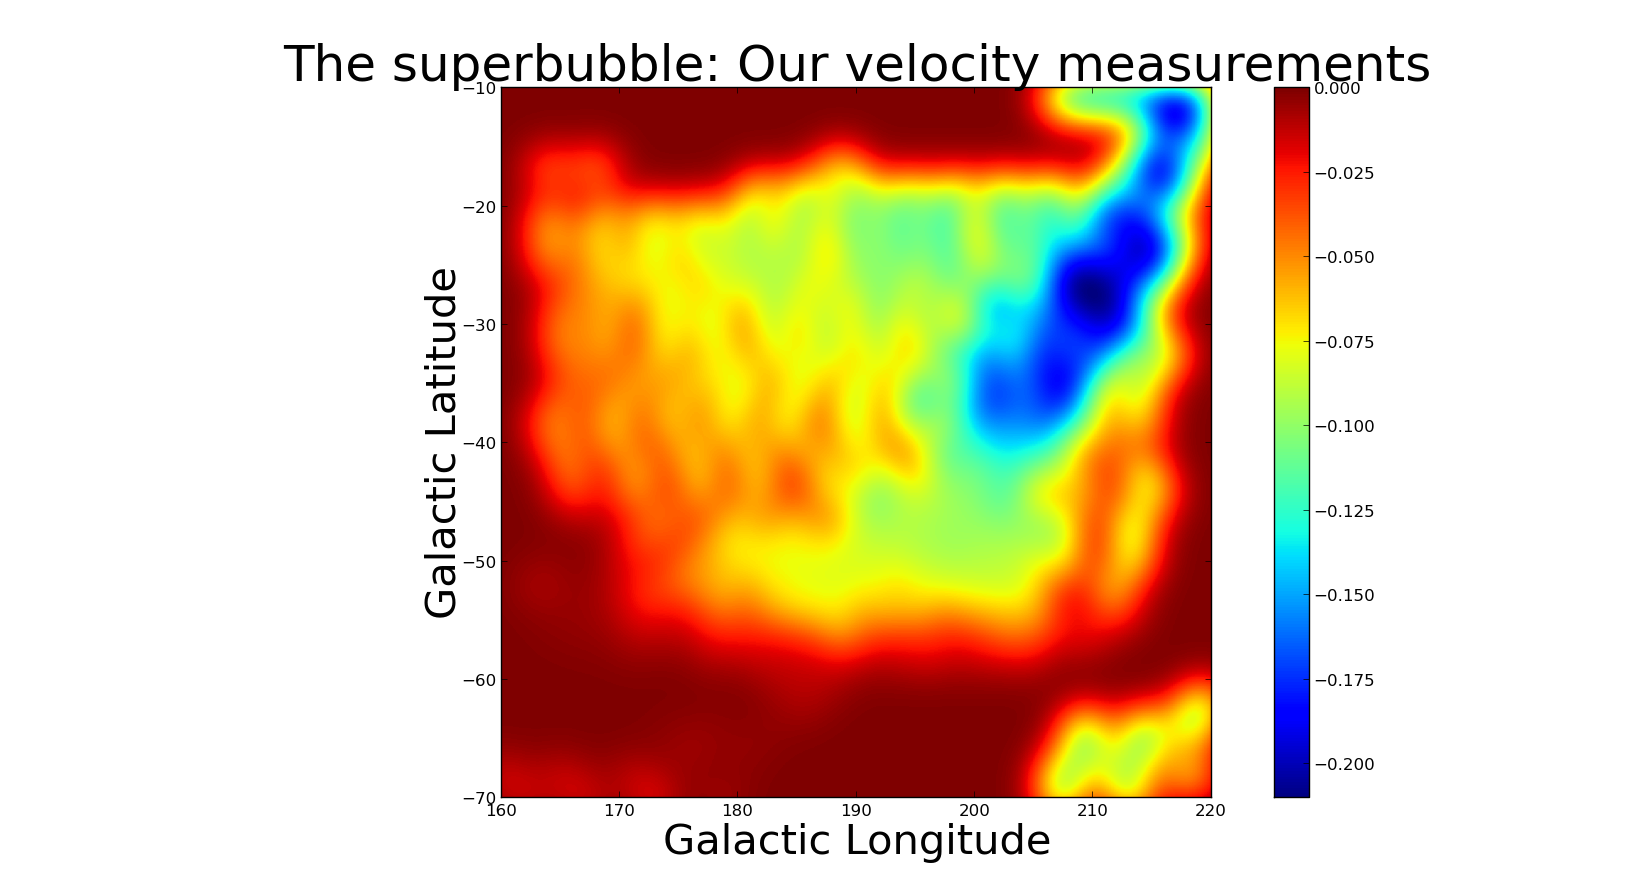
\includegraphics[scale=0.35]{garphs/velocity}
\caption{This graph maps the velocities of areas of the Orion-Eridanus superbubble as a function of latitude and longitude. We smoothed using a Gaussian centered in the center of the screen with standard deviation 3.1 degrees. Redder regions are moving faster in our direction. As above, only the relative measurements have significance.\label{velocity}}
\end{figure} 

The velocity dispersion of the observable parts of the bubble is predominantly in our direction; this is because the bubble is expanding, so the parts we see are getting closer to us, even though the universe is expanding. We can compare the figures generated by our plots to a reference image of the bubble published in ``The Orion OB1 Association'', an article by AGA Brown, D Hartmann, and WB Burton in the 1995 issue of the journal Astronomy and Astrophysics. This appears in Figure \ref{canon}.

\begin{figure}
\centering
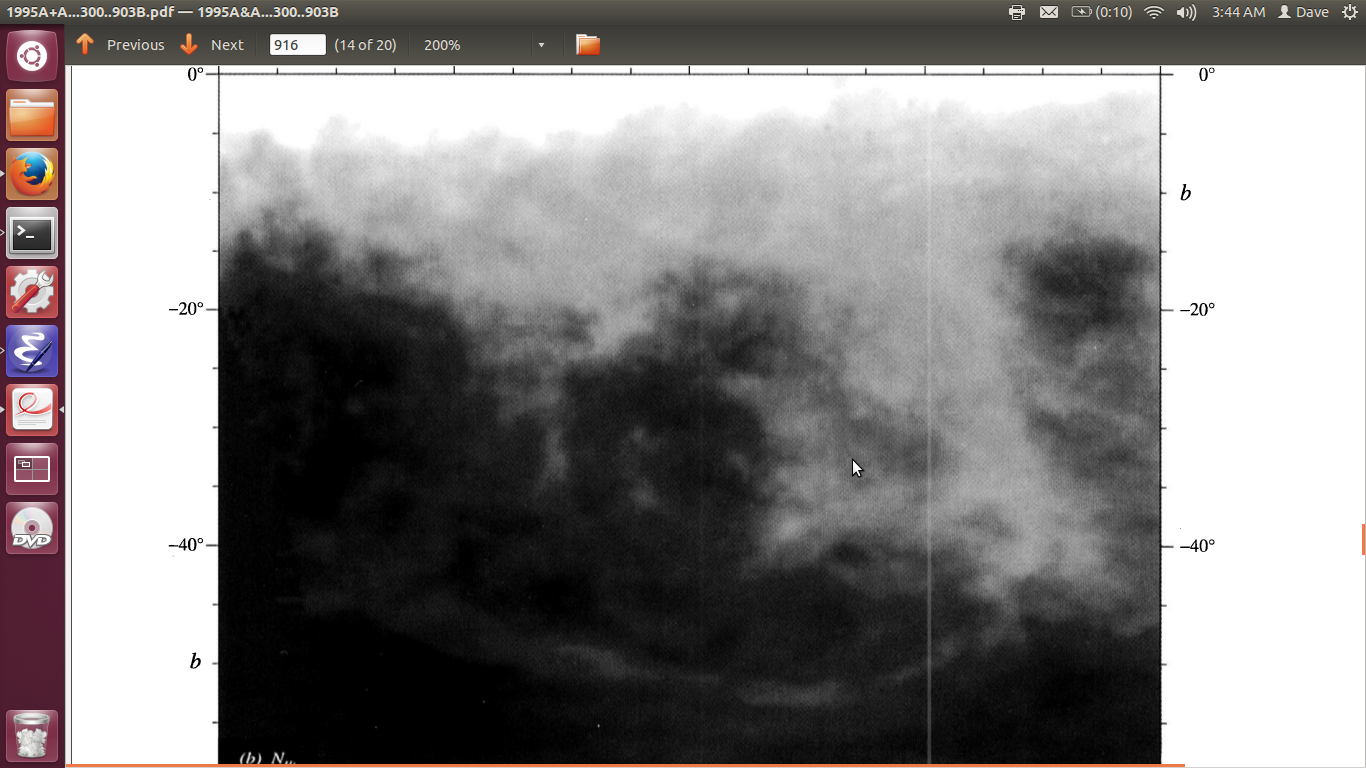
\includegraphics[scale=0.35]{garphs/superbubble}
\caption{This is what the superbubble looks like with a better telescope, longer integration time, and/or more pointings.  \label{canon}}
\end{figure} 

Comparing Figure \ref{canon} with Figure \ref{hydrogen}, we can see unmistakable similarities. Differences in graphing procedures have resulted in our image seeming to capture a mirror reflection of the reference image. Mentally flipping the reference image, one can see that the high-denstiy regions line up nicely with our high-density regions, at least on the largest scales, and we capture some of the smaller-scale structure too. In places where we don't have any pointings, of course, our perceived density is much lower than the actual density. 

\section{Conclusion}
In conclusion, this was a really cool lab. We got to see a really big bubble, and we learned a lot about science in the process. Sadly, a late start and technical difficulties conspired to provide us with half the number of telescope pointings we were wanting to take, so given more time we would take the rest of those pointings and complete the picture of the bubble. 
%COMMENT: In a report you don't need to write out unit names, and it
%would actually be preferred you use things like $\mu$H versus mircoHenry
\section{Acknowledgements}
My partners were Kyle, Leonardo, and Eduardo. We made a super awesome team!
\end{document}
